\begin{figure}
	\centering
	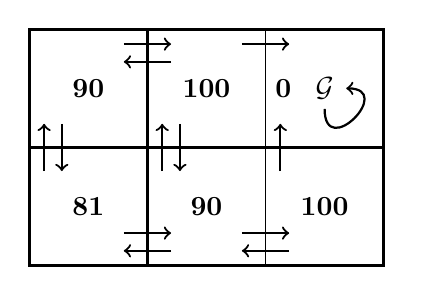
\begin{tikzpicture}[scale=0.75]
	
		\draw[very thick] (0,0) -- (6,0) -- (6,4) -- (0,4) -- cycle;
		\draw[thick] (2,0) -- (2,4); \draw (4,0) -- (4,4);
		\draw[thick] (0,2) -- (6,2);

		\draw[->,thick] (1.6,3.75) -- (2.4,3.75);
		\draw[->,thick] (2.4,3.45) -- (1.6,3.45);

		\draw[->,thick] (1.6,0.55) -- (2.4,0.55);
		\draw[->,thick] (2.4,0.25) -- (1.6,0.25);

		\draw[->,thick] (3.6,0.55) -- (4.4,0.55);
		\draw[->,thick] (4.4,0.25) -- (3.6,0.25);

		\draw[->,thick] (0.25,1.6) -- (0.25,2.4);
		\draw[->,thick] (0.55,2.4) -- (0.55,1.6);

		\draw[->,thick] (2.25,1.6) -- (2.25,2.4);
		\draw[->,thick] (2.55,2.4) -- (2.55,1.6);

		\draw[->,thick] (3.6,3.75) -- (4.4,3.75);
		\draw[->,thick] (4.25,1.6) -- (4.25,2.4);

		\node (G) at (5,3) {$\bm{\mathcal{G}}$};
		\draw[thick,->,shorten >=1pt] (G) to [out=270,in=360,loop,looseness=4.8] (G);
		\node at (4.3,3) {\textbf{0}};

		\node at (1, 1) {\textbf{81}};
		\node at (3, 1) {\textbf{90}};
		\node at (5, 1) {\textbf{100}};

		\node at (1, 3) {\textbf{90}};
		\node at (3, 3) {\textbf{100}};
	
	\end{tikzpicture}
\end{figure}